
\thispagestyle{empty}
%\put(0,0){
\begin{minipage}[h]{0.9\paperwidth}
\thispagestyle{empty}
\begin{tikzpicture}[remember picture,overlay]
\node (f) [rectangle]  
at (current page.center)
          {\parbox[b][\paperheight]{\paperwidth}{
           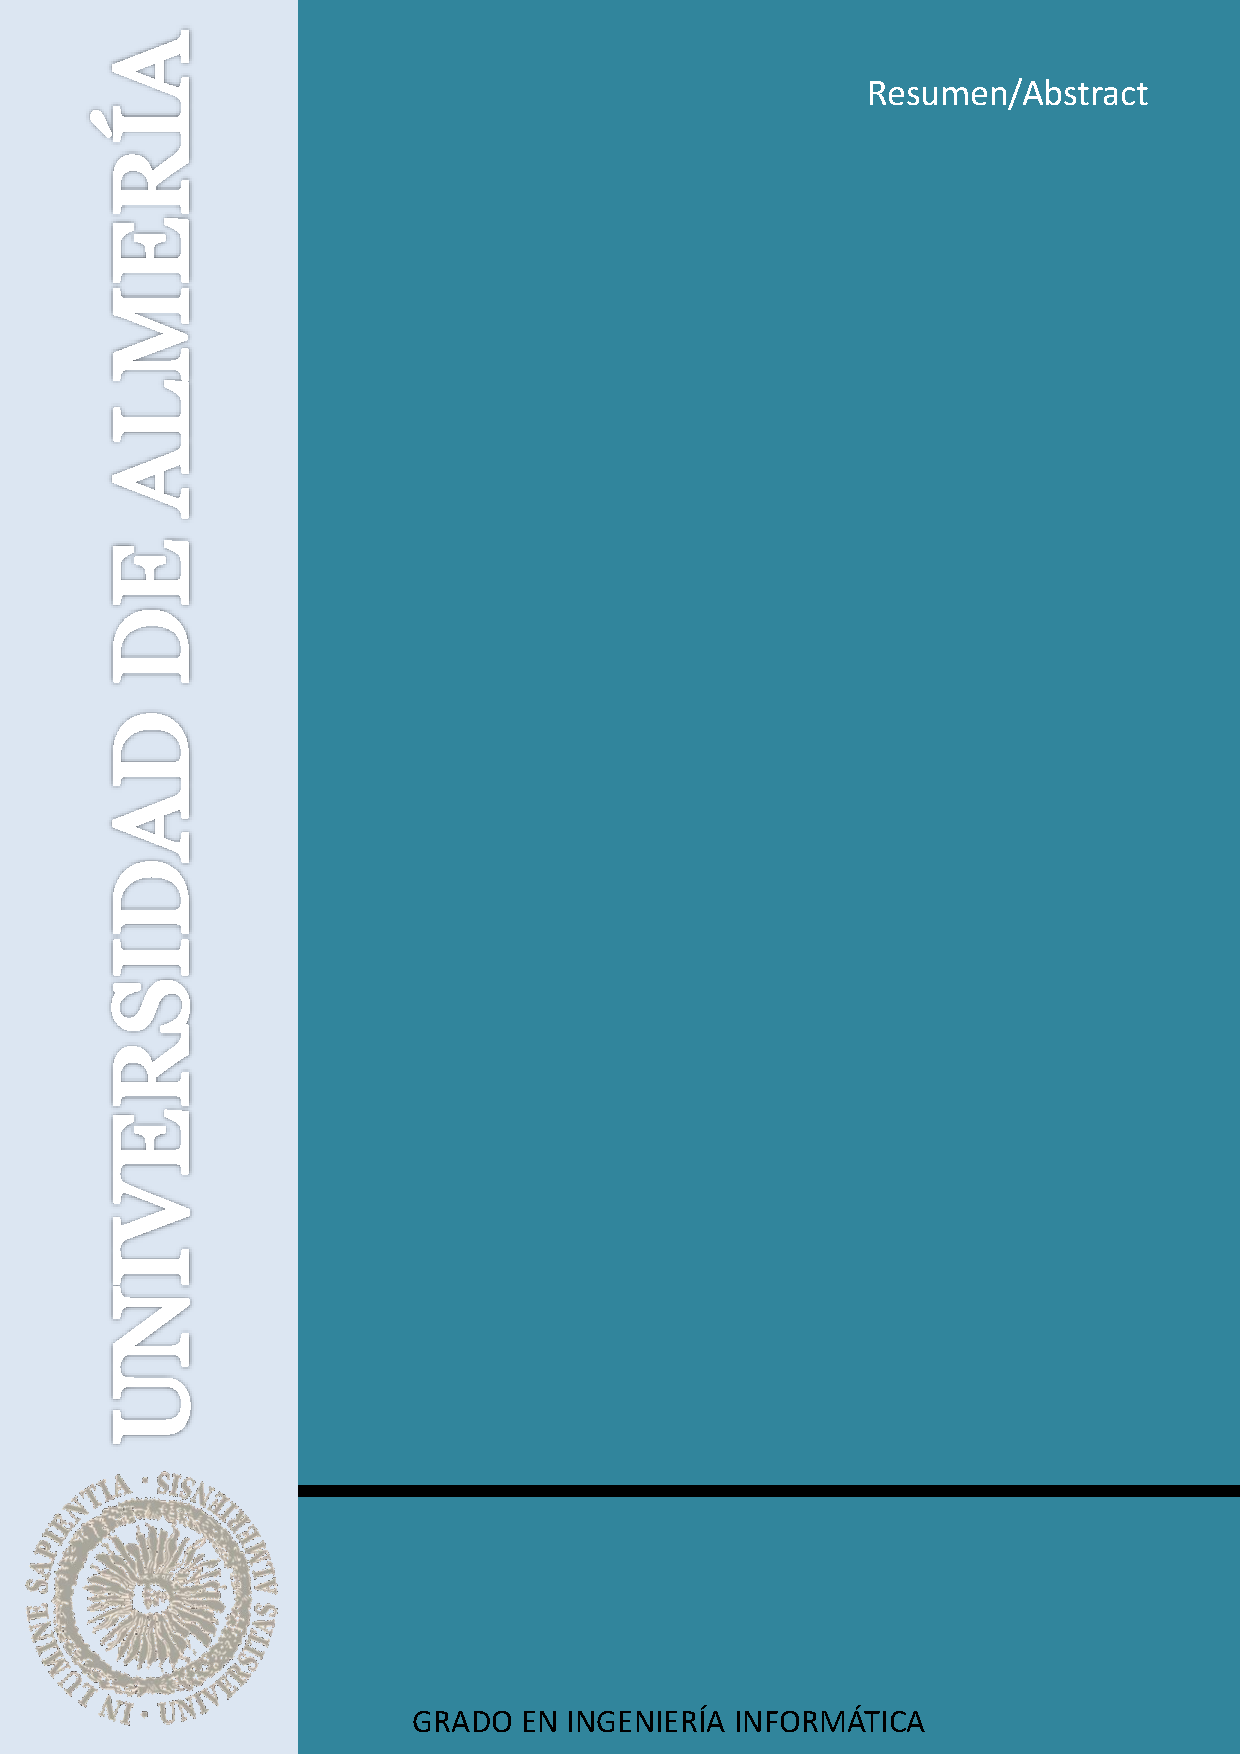
\includegraphics[width=\paperwidth,height=\paperheight,keepaspectratio]{Figuras/logos/TFG_back}
          }};
\node (texto) [rectangle,text width=0.5\paperwidth,yshift=50pt] 
at (f)
          {\parbox{0.65\paperwidth}{\justifying \Large \color{white}
         
\normalsize {}	
Actualmente, las organizaciones comienzan a implementar un nuevo modelo de marketing
centrado en las relaciones entre la empresa y sus clientes. La inteligencia artificial ha encontrado aquí un extraordinario campo de aplicación, tanto en la gestión de la información, como en la atención al cliente y el análisis de la experiencia de compra.

El proyecto desarrollado en el presente trabajo se sitúa en este contexto. Se estudian e implementan dos servicios de inteligencia artificial en una tienda electrónica. Por un lado, se construye una aplicación basada en Google Natural Language que realiza un análisis de sentimientos de los comentarios de los clientes, proporcionando una medida normalizada de su grado de satisfacción sobre el servicio ofrecido. Por otro lado, se desarrolla un agente virtual utilizando Dialogflow para ayudar al servicio de atención al cliente, automatizando las tareas más sencillas.

El sistema de software implementado se despliega a través de contenedores en Cloud Run, una plataforma sin servidor que permite a las organizaciones abstraerse de cuestiones técnicas relacionadas con la infraestructura, flexibilidad y disponibilidad de recursos.

\vspace{.5cm}

Palabras clave: Comercio electrónico, machine learning, chatbots, computación en la nube, análisis de sentimientos.

\vspace{1cm}

\newpage
 
%\section*{Abstract}

Nowadays, corporations are beginning to implement a new marketing that pays closer attention to their relationship with clients. In this area, Artificial Intelligence has found new fields of application such as data management, customer service or shopping experience analysis.

The project developed in the current work is situated in this context. Two AI services have been studied and implemented in an e-commerce. First of all, an app based on Google Natural Language has been built, it will carry out a sentiment analysis of customer feedback, providing a standardized measure of the satisfaction degree about the service offered. Second, a virtual agent has been developed using Dialogflow to help customer service by automating simple tasks.

To conclude, the system is deployed through containers on Cloud Run, a serverless platform that allows organizations to abstract from technical issues related to infrastructure, flexibility, and resource availability.

\vspace{.5cm}

Keywords: E-commerce, machine learning, chatbots, cloud computing, sentiment analysis.

         }};
       \node  at (14,-25.55) {\Large\curso};
  \end{tikzpicture}
\end{minipage}
%}


          
          